\chapter{モジュライ空間と幾何学的自由度}
\label{ch:ch16}

\begin{chapterlead}
弦理論のコンパクト化では，内部空間 $X$ の「形」と「大きさ」は固定された背景ではなく，4次元時空の場として振る舞う．
本章では，幾何学的対象を同型を除いて分類する空間＝\textbf{モジュライ空間}の考え方を導入し，
変形理論（Kodaira--Spencer 理論）によってその局所構造を調べる．
最後に Calabi--Yau 多様体の複素構造モジュライと K\"ahler モジュライを詳しく調べ，
それらが 4 次元有効理論の質量ゼロのスカラー場（モジュライ場）として現れることを見る．
Calabi--Yau 多様体の定義・Hodge 数・具体例は第15章で，ベクトル束や Higgs 束のモジュライは第14章で扱った．
\end{chapterlead}

%======================================================================
\section{モジュライの基本概念}
%======================================================================

\subsection{モジュライ問題}

代数幾何学の多くの問いは，次の形にまとめられる．

\begin{quote}
ある種類の幾何学的対象（曲線，曲面，ベクトル束，部分多様体，$\dots$）を，同型を除いて分類せよ．
\end{quote}

分類が有限個の離散的な不変量で済むことはまれで，多くの場合，分類は\textbf{連続パラメータ}を含む．
例えば種数 $1$ の曲線（楕円曲線）は位相的にはすべてトーラスであるが，複素多様体としては 1 個の複素パラメータ $\tau$ に依存する族をなし，$\tau$ の値が違えば一般に同型でない．
このような「連続的に変わる分類パラメータ」をモジュライ（moduli）とよぶ．この語は Riemann が種数 $g$ の Riemann 面が $3g-3$ 個の複素パラメータ（moduli）に依存すると述べたことに由来する．

\begin{mydef}{モジュライ問題（素朴な形）}{ch16-moduli-problem}
幾何学的対象のクラス $\mathcal{C}$ と，その上の同値関係 $\sim$（通常は同型）が与えられたとき，
集合 $\mathcal{C}/\!\sim$ に自然な幾何学的構造（多様体，スキーム，$\dots$）を入れ，
その点が対象の同値類と 1 対 1 に対応し，かつ「対象の連続的な族」が「その空間への連続的（代数的）な写像」に対応するようにせよ，という問題を\textbf{モジュライ問題}といい，そのような空間 $\mathcal{M}$ を\textbf{モジュライ空間}という．
\end{mydef}

「点が同値類と 1 対 1 に対応する」だけなら単なる集合であり，意味のある条件は後半の「族との対応」である．これを正確に述べるには族の概念が必要になる．

\begin{mydef}{族}{ch16-family}
基底 $B$（多様体またはスキーム）上の $\mathcal{C}$ の\textbf{族}とは，平坦な射 $\pi:\mathcal{X}\to B$ であって，各ファイバー $X_b=\pi^{-1}(b)$ が $\mathcal{C}$ に属するものをいう．
二つの族 $\mathcal{X}\to B$, $\mathcal{X}'\to B$ が同型とは，$B$ 上の同型 $\mathcal{X}\cong \mathcal{X}'$ が存在することをいう．
また $f:B'\to B$ に対し，ファイバー積 $f^*\mathcal{X}=\mathcal{X}\times_B B'\to B'$ を\textbf{引き戻し}の族という．
\end{mydef}

\begin{mydef}{細モジュライ空間と粗モジュライ空間}{ch16-fine-coarse}
基底 $B$ に $B$ 上の族の同型類の集合を対応させる（反変）関手を
\[
\mathfrak{M}(B)=\{\,B \text{ 上の } \mathcal{C} \text{ の族}\,\}/\cong
\]
とおく．
\begin{enumerate}
\item 空間 $\mathcal{M}$ と族 $\mathcal{U}\to\mathcal{M}$（\textbf{普遍族}）があって，任意の族 $\mathcal{X}\to B$ に対し $\mathcal{X}\cong f^*\mathcal{U}$ となる射 $f:B\to\mathcal{M}$ がただ一つ存在するとき（すなわち $\mathfrak{M}\cong \Hom(-,\mathcal{M})$ と表現可能なとき），$\mathcal{M}$ を\textbf{細モジュライ空間}(fine moduli space)という．
\item 普遍族は存在しないが，自然変換 $\mathfrak{M}\to\Hom(-,\mathcal{M})$ があって，(a) $\C$ 値点 $\mathfrak{M}(\mathrm{pt})\to\mathcal{M}(\C)$ が全単射，(b) この性質を持つ空間の中で普遍的，を満たすとき，$\mathcal{M}$ を\textbf{粗モジュライ空間}(coarse moduli space)という．
\end{enumerate}
\end{mydef}

\begin{note}
細モジュライ空間が存在しない典型的な原因は\textbf{自己同型}である．
対象 $X$ が非自明な自己同型 $\sigma$ を持つと，$X\times[0,1]$ の両端を $\sigma$ で貼り合わせた族（円周 $S^1$ 上の族）は，すべてのファイバーが $X$ と同型なのに族として自明でない．
細モジュライ空間があれば，この族は定値写像 $S^1\to\mathcal{M}$ の引き戻し，すなわち自明族でなければならず矛盾する．
楕円曲線は常に自己同型 $P\mapsto -P$ を持つので，楕円曲線の細モジュライ空間（スキームとして）は存在しない．
これを解決する一つの方法は，自己同型を「覚えている」空間＝\textbf{スタック}（代数スタック，orbifold）を用いることである．本ノートではスタック論には立ち入らず，粗モジュライ空間に orbifold 構造を付加して考える．
\end{note}

\subsection{幾何学的対象の分類}

分類には二つの段階がある．
\begin{enumerate}
\item \textbf{離散不変量}による大分類：次元，種数，次数，Chern 類，Hodge 数，Hilbert 多項式など．これらは連続変形で変わらない．
\item 離散不変量を固定したうえでの\textbf{連続的な分類}：これがモジュライ空間である．
\end{enumerate}
例えばコンパクト Riemann 面（＝滑らかな射影代数曲線）は種数 $g$ で位相的に分類され，種数 $g$ を固定したモジュライ空間 $\mathcal{M}_g$ の次元は
\[
\dim_\C \mathcal{M}_0=0,\qquad \dim_\C\mathcal{M}_1=1,\qquad \dim_\C\mathcal{M}_g=3g-3\ (g\ge2)
\]
である（$\mathcal{M}_1$ は印付き点も込めて $\mathcal{M}_{1,1}$ と書くのが普通である）．この次元は 16.2 節で変形理論から導く．

\subsection{同値関係による分類}

モジュライ空間の多くは，「対象を具体的に記述するデータの空間 $P$」を「同じ対象を与えるデータを同一視する群作用」で割った商 $P/G$ として得られる．
例えば射影空間内の超曲面は定義多項式の係数で記述でき，射影変換で移り合う超曲面は同型であるから，
\[
\{\text{超曲面}\}/\cong \;\approx\; \PP(\text{係数の空間})^{\text{滑らか}}/\PGL(n+1,\C)
\]
という形の記述を得る（「$\approx$」としたのは，抽象的な同型が射影変換から来るかどうかは別に確かめる必要があるからである．次数 $\ge 3$ の滑らかな超曲面では，例外を除き正しい）．

商空間 $P/G$ が良い空間になるとは限らない．
軌道が閉じていない（ある軌道の閉包に別の軌道が含まれる）と，商位相が Hausdorff でなくなる．
この問題を代数的に処理するのが Mumford の\textbf{幾何学的不変式論}(GIT)であり，「安定」な点だけを残すことで良い商を作る．第14章で見たベクトル束の安定性条件はこの考え方の現れである．

\begin{myex}{非 Hausdorff な商}{ch16-nonhausdorff}
$\C^*$ が $\C^2$ に $t\cdot(x,y)=(tx,t^{-1}y)$ で作用するとする．軌道は
双曲線 $\{xy=c\}$ ($c\neq0$)，$x$ 軸から原点を除いたもの，$y$ 軸から原点を除いたもの，原点
の 4 種類である．$c\to0$ のとき双曲線は $x$ 軸・$y$ 軸・原点のすべてに近づくので，商空間ではこの 3 点を分離できない．
不変式 $xy$ で $\C^2\to\C$ を作ると（GIT 商 $\C^2/\!\!/\C^*=\C$），$c=0$ の 3 つの軌道は 1 点につぶれる．
\end{myex}

\subsection{パラメータ空間とモジュライ空間}

\begin{mydef}{パラメータ空間}{ch16-parameter-space}
クラス $\mathcal{C}$ の対象を（冗長性を許して）すべて含む族 $\mathcal{X}\to P$ があり，同型な対象を与える点同士が群 $G$ の作用で移り合うとき，$P$ を\textbf{パラメータ空間}という．このときモジュライ空間は（存在すれば）$\mathcal{M}=P/G$ で与えられ，
\[
\dim\mathcal{M}=\dim P-\dim G+\dim(\text{一般の点の固定化群})
\]
が成り立つ．
\end{mydef}

\begin{myex}{平面円錐曲線}{ch16-conics}
$\PP^2$ 内の円錐曲線（2次曲線）は
\[
C:\ a_0x^2+a_1y^2+a_2z^2+a_3xy+a_4yz+a_5zx=0
\]
で与えられ，係数はスカラー倍を除いて決まるので，円錐曲線全体のパラメータ空間は $P=\PP^5$ である．
対称行列
\[
A=\begin{pmatrix} a_0 & a_3/2 & a_5/2\\ a_3/2 & a_1 & a_4/2\\ a_5/2 & a_4/2 & a_2\end{pmatrix}
\]
を用いれば $C=\{\,{}^t\!v Av=0\,\}$ であり，$C$ が滑らか $\iff \det A\neq0$ である．
したがって特異な円錐曲線全体は 3 次超曲面 $\{\det A=0\}\subset\PP^5$（判別式超曲面）であり，その中で $\rank A=1$（重複直線）の部分は Veronese 曲面 $\cong\PP^2$ である．

$\PGL(3,\C)$ は $A\mapsto {}^t\!gAg$ で作用し，複素対称行列は正則行列による合同変換で単位行列に移せるから，\textbf{滑らかな円錐曲線はすべて射影同値}である．
次元を数えると，$\dim\PGL(3)=8$，$x^2+y^2+z^2=0$ の固定化群は $\mathrm{PO}(3,\C)$ で次元 $3$ だから，軌道の次元は $8-3=5=\dim\PP^5$．よって滑らかな円錐曲線のモジュライ空間は 1 点である（実際，滑らかな円錐曲線はすべて $\PP^1$ と同型）．
\end{myex}

\begin{myex}{平面 3 次曲線}{ch16-cubics}
$\PP^2$ 内の 3 次曲線の係数は $\binom{3+2}{2}=10$ 個なので $P=\PP^9$．
$\PGL(3)$ の次元は $8$ で，一般の滑らかな 3 次曲線の射影変換による固定化群は有限群である．よって
\[
\dim\mathcal{M}=9-8=1 .
\]
滑らかな平面 3 次曲線は楕円曲線であり（第13章），この 1 次元が下で見る $\mathcal{M}_{1,1}$ の次元である．
\end{myex}

\subsection{モジュライ空間の基本例}

最も重要な基本例は楕円曲線のモジュライ空間 $\mathcal{M}_{1,1}$ である．
第13章で見たように，楕円曲線は格子 $\Lambda\subset\C$ による商 $E=\C/\Lambda$ として表される．
$\Lambda=\Z\omega_1+\Z\omega_2$ で $\Img(\omega_2/\omega_1)>0$ となるよう基底をとり，$\C$ の相似変換 $z\mapsto z/\omega_1$ で正規化すると $\Lambda=\Z+\Z\tau$，$\tau\in\mathbb{H}=\{\tau\in\C\mid \Img\tau>0\}$ を得る．

\begin{myprop}{楕円曲線の同型類}{ch16-elliptic-iso}
$E_\tau=\C/(\Z+\Z\tau)$ と $E_{\tau'}$ が（原点を保つ）複素多様体として同型であるための必要十分条件は，
\[
\tau'=\frac{a\tau+b}{c\tau+d},\qquad \begin{pmatrix}a&b\\c&d\end{pmatrix}\in\SL(2,\Z)
\]
となることである．したがって
\[
\mathcal{M}_{1,1}=\mathbb{H}/\SL(2,\Z)\qquad(\text{実質的には } \mathbb{H}/\mathrm{PSL}(2,\Z)) .
\]
\end{myprop}

\begin{proof}[証明の概略]
同型 $E_\tau\to E_{\tau'}$ は普遍被覆 $\C$ 上の正則写像に持ち上がり，原点を保つ双正則写像は $z\mapsto\alpha z$ ($\alpha\in\C^*$) の形をしている（$\C$ 上の正則関数で微分が格子周期的なもの，すなわち定数）．よって $\alpha(\Z+\Z\tau)=\Z+\Z\tau'$．
これは $\alpha\tau=a\tau'+b$, $\alpha=c\tau'+d$ と書けて行列が $\GL(2,\Z)$ に属することを意味し，両辺の比をとれば $\tau=(a\tau'+b)/(c\tau'+d)$．$\Img$ の符号を保つ条件から行列式は $+1$ である．逆も同様．$-1\in\SL(2,\Z)$ は $\mathbb{H}$ に自明に作用し，$E$ の自己同型 $z\mapsto -z$ に対応する．
\end{proof}

$\SL(2,\Z)$ は $T=\begin{pmatrix}1&1\\0&1\end{pmatrix}$ ($\tau\mapsto\tau+1$) と $S=\begin{pmatrix}0&-1\\1&0\end{pmatrix}$ ($\tau\mapsto-1/\tau$) で生成され，その作用の\textbf{基本領域}として
\[
\mathcal{F}=\Bigl\{\tau\in\mathbb{H}\ \Big|\ |\Re\tau|\le\tfrac12,\ |\tau|\ge1\Bigr\}
\]
がとれる（境界は $T$ と $S$ で同一視される）．図 \ref{fig:ch16-fundamental-domain} を参照．

\begin{figure}[H]
\centering
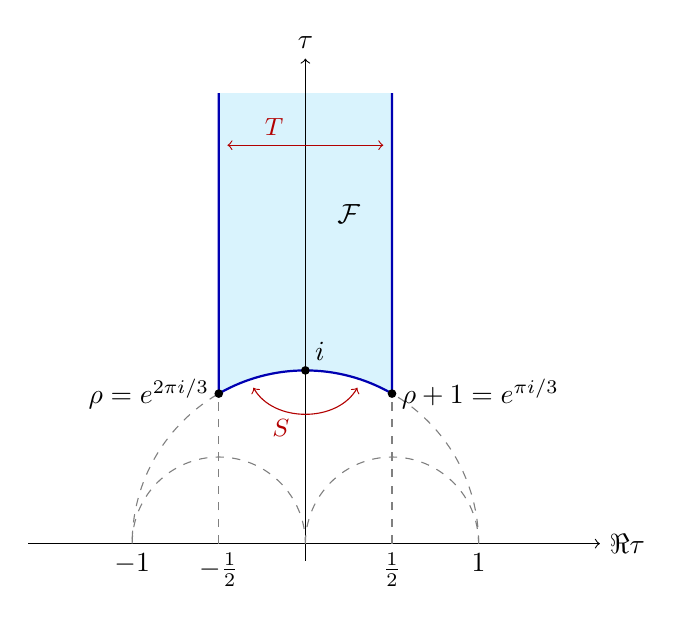
\begin{tikzpicture}[scale=2.2]
  % shaded fundamental domain
  \fill[cyan!15] (-0.5,0.866) arc (120:60:1) -- (0.5,2.6) -- (-0.5,2.6) -- cycle;
  \draw[->] (-1.6,0) -- (1.7,0) node[right] {$\Re\tau$};
  \draw[->] (0,-0.1) -- (0,2.8) node[above] {$\Img\tau$};
  \draw[gray,dashed] (1,0) arc (0:180:1);
  \draw[gray,dashed] (-0.5,0) -- (-0.5,0.866);
  \draw[gray,dashed] (0.5,0) -- (0.5,0.866);
  \draw[gray,dashed] (0,0) arc (180:0:0.5);
  \draw[gray,dashed] (-1,0) arc (180:0:0.5);
  \draw[thick,blue!70!black] (-0.5,2.6) -- (-0.5,0.866) arc (120:60:1) -- (0.5,2.6);
  \fill (0,1) circle (0.025) node[above right] {$i$};
  \fill (-0.5,0.866) circle (0.025) node[left] {$\rho=e^{2\pi i/3}$};
  \fill (0.5,0.866) circle (0.025) node[right] {$\rho+1=e^{\pi i/3}$};
  \node at (0.25,1.9) {$\mathcal{F}$};
  \node[below] at (-0.5,0) {$-\frac12$};
  \node[below] at (0.5,0) {$\frac12$};
  \node[below] at (1,0) {$1$};
  \node[below] at (-1,0) {$-1$};
  \draw[<->,red!70!black] (-0.45,2.3) -- node[pos=0.3,above] {\small $T$} (0.45,2.3);
  \draw[<->,red!70!black] (-0.3,0.9) to[bend right=60] node[pos=0.3,below] {\small $S$} (0.3,0.9);
\end{tikzpicture}
\caption{$\SL(2,\Z)$ の $\mathbb{H}$ への作用の基本領域 $\mathcal{F}$．左右の縦の辺は $T$ で，単位円上の弧は $S$ で（$i$ を中心に折り返して）同一視される．$i$ と $\rho=e^{2\pi i/3}$ では固定化群がそれぞれ位数 $4$，$6$ に大きくなり（$\pm1$ を含めて），$\mathcal{M}_{1,1}$ の orbifold 点となる．}
\label{fig:ch16-fundamental-domain}
\end{figure}

境界の同一視を行うと $\mathcal{F}$ は穴あき球面（cusp $\tau\to i\infty$ を除いた球面）と同相になる．
これを複素多様体として具体的に実現するのが j 不変量である（第13章では結果のみ述べた）．

\begin{mydef}{j 不変量}{ch16-j-invariant}
$\tau\in\mathbb{H}$ に対し，Eisenstein 級数 $G_{2k}(\tau)=\sum_{(m,n)\neq(0,0)}(m+n\tau)^{-2k}$ を用いて
\[
g_2(\tau)=60\,G_4(\tau),\qquad g_3(\tau)=140\,G_6(\tau),\qquad \Delta(\tau)=g_2^3-27g_3^2,
\]
\[
j(\tau)=1728\,\frac{g_2(\tau)^3}{\Delta(\tau)}
\]
と定める．$j(\tau)$ を \textbf{j 不変量}（楕円モジュラー関数）という．
\end{mydef}

\begin{mythm}{$\mathcal{M}_{1,1}$ の粗モジュライ空間}{ch16-j-line}
$j:\mathbb{H}\to\C$ は $\SL(2,\Z)$ 不変な正則関数であり，全単射
\[
j:\ \mathbb{H}/\SL(2,\Z)\ \xrightarrow{\ \sim\ }\ \C
\]
を誘導する．したがって楕円曲線の粗モジュライ空間は複素アフィン直線 $\A^1_j$ であり，$q=e^{2\pi i\tau}$ を用いれば
\[
j(\tau)=\frac1q+744+196884\,q+21493760\,q^2+\cdots
\]
と展開される．特別な値は $j(i)=1728$，$j(\rho)=0$ ($\rho=e^{2\pi i/3}$) である．
\end{mythm}

\begin{proof}[証明の概略]
$G_{2k}(\tau)$ は重さ $2k$ のモジュラー形式：$G_{2k}\bigl(\tfrac{a\tau+b}{c\tau+d}\bigr)=(c\tau+d)^{2k}G_{2k}(\tau)$．
よって $g_2^3$ と $\Delta$ はともに重さ $12$ で，比 $j$ は重さ $0$，すなわち不変である．$\Delta$ は $\mathbb{H}$ 上零点を持たない（$\Delta\ne0$ は Weierstrass 3 次式が重根を持たないこと，第13章）．$q$ 展開では $\Delta=(2\pi)^{12}q\prod(1-q^n)^{24}$ が $q$ の 1 位の零点を持つので $j$ は cusp で 1 位の極を持つ．基本領域の境界を周回する積分で零点を数える標準的な議論（「$k/12$ 公式」）により，各 $c\in\C$ に対し $j(\tau)=c$ は $\mathcal{F}$ 内（同一視込み）でちょうど 1 つの解を持つ．
$\tau=i$ は $S$ で固定され $g_3(i)=i^{6}g_3(i)=-g_3(i)$ より $g_3(i)=0$，よって $j(i)=1728$．
$\tau=\rho$ は $ST$ の固定点で同様に $g_2(\rho)=0$，よって $j(\rho)=0$．
\end{proof}

\begin{physbox}[モジュライ空間の特異点]
$\mathcal{M}_{1,1}$ は粗モジュライ空間としては滑らかな $\C$ であるが，$j=1728,0$ の点では対応する楕円曲線が余分な自己同型（$z\mapsto iz$, $z\mapsto\rho z$）を持ち，orbifold としては $\Z_2,\Z_3$ 型の錐点（$\pm1$ を除いて）を持つ．
物理では，モジュライ空間上の「対称性が増大する点」はしばしば新しい質量ゼロの状態やゲージ対称性の増大と結び付く．
またトーラス上の 2 次元 CFT の分配関数がモジュラー不変であること（13.6.4 項，17.1.5 項）は，$\tau$ と $\gamma\tau$ が同じ物理を表すこと，すなわち物理的なパラメータ空間が $\mathbb{H}$ ではなく $\mathbb{H}/\SL(2,\Z)$ であることの表れである．
\end{physbox}

\exprob{prob:ch16-1-1}
$\PP^3$ 内の滑らかな 4 次曲面（K3 曲面）全体を考える．4 次斉次多項式の係数の個数と $\PGL(4,\C)$ の次元から，4 次曲面のモジュライ空間の次元を求めよ．ただし一般の滑らかな 4 次曲面の射影変換による固定化群は有限であることを用いてよい．

\exprob{prob:ch16-1-2}
$\SL(2,\Z)$ の作用で $\tau=i$ を固定する元，$\tau=\rho=e^{2\pi i/3}$ を固定する元をすべて求め，それぞれの固定化群が位数 $4$, $6$ の巡回群であることを示せ．また，$j(\tau)-1728$ が $\tau=i$ で（$\tau$ の関数として）2 位の零点を持つことを，この固定化群を用いて説明せよ．

%======================================================================
\section{幾何学的構造の変形}
%======================================================================

\subsection{変形の概念}

モジュライ空間の大域的構造を知ることは一般に難しい．しかし与えられた点 $[X]\in\mathcal{M}$ の\textbf{近傍}の構造，すなわち「$X$ を少しだけ変えるとどうなるか」は線形代数（コホモロジー）で調べることができる．これが\textbf{変形理論}である．

\begin{mydef}{変形}{ch16-deformation}
コンパクト複素多様体 $X$ の\textbf{変形}とは，連結な基底 $(B,0)$ 上の固有で滑らかな（沈め込みである）正則写像 $\pi:\mathcal{X}\to B$ と同型 $\iota:X\xrightarrow{\sim}\pi^{-1}(0)$ の組をいう．
特に $B=\Spec\C[\varepsilon]/(\varepsilon^2)$ のときを\textbf{一次変形}（無限小変形）という．
\end{mydef}

一次変形は「$\varepsilon$ の 1 次まで」の変形であり，物理での摂動の 1 次に相当する．

\subsection{幾何学的構造の連続変形}

Ehresmann の定理により，固有な沈め込み $\pi:\mathcal{X}\to B$ は $C^\infty$ 級には局所自明である．すなわち $0$ の近傍で $\mathcal{X}\cong X\times B$（可微分同相）となる．したがって変形の族では，\textbf{下にある可微分多様体 $M$ は変わらず，その上の複素構造だけが変わる}と考えてよい．
これは物理的にも自然な見方で，例えば内部空間の位相（Hodge 数・交点数など）は変わらず，計量や複素構造が連続的に動く．

複素構造は，概複素構造 $J:TM\to TM$ ($J^2=-1$) で可積分なもの（Newlander--Nirenberg）として与えられる．
$J$ を変えることは，$(0,1)$ 型ベクトルの部分空間 $T^{0,1}$ を変えることと同じで，小さな変形は
\[
T^{0,1}_{\phi}=\{\,\bar v+\phi(\bar v)\mid \bar v\in T^{0,1}\,\},\qquad \phi\in A^{0,1}(X,T_X)
\]
と，$T_X=T^{1,0}$ に値をとる $(0,1)$ 形式 $\phi=\phi^{i}{}_{\bar j}\,d\bar z^{j}\otimes\partial_i$ で記述される（Beltrami 微分）．

\subsection{複素構造の変形}

\begin{mythm}{Kodaira--Spencer}{ch16-kodaira-spencer}
コンパクト複素多様体 $X$ について次が成り立つ．
\begin{enumerate}
\item $X$ の一次変形の同型類は $H^1(X,T_X)$ と自然に 1 対 1 に対応する．
\item 変形の族 $\pi:\mathcal{X}\to B$ に対し，\textbf{Kodaira--Spencer 写像}
\[
\kappa_b:\ T_bB\longrightarrow H^1(X_b,T_{X_b})
\]
が定まり，これは族を接ベクトル方向に一次で制限したものの類を与える．
\item 一次変形を高次に延長できるかどうかの\textbf{障害}は $H^2(X,T_X)$ に値をとる．特に $H^2(X,T_X)=0$ なら障害はない．
\end{enumerate}
\end{mythm}

\begin{proof}[証明の概略]
(1) $X$ を座標近傍 $\{U_i\}$ で覆い，変形 $\mathcal{X}_\varepsilon$ を $U_i\times\Spec\C[\varepsilon]/(\varepsilon^2)$ を貼り合わせて作る．貼り合わせ写像は恒等写像の一次の摂動
\[
z_i=f_{ij}(z_j)+\varepsilon\,\theta_{ij}(z_j)\cdot\partial f_{ij},\qquad \theta_{ij}\in\Gamma(U_{ij},T_X)
\]
の形をしており，貼り合わせの整合性（三重交差での一致）は $\theta_{ij}+\theta_{jk}+\theta_{ki}=0$，すなわち $\{\theta_{ij}\}$ が \v{C}ech 1-コサイクルであることと同値である．
各 $U_i$ の座標を $z_i\mapsto z_i+\varepsilon\,\eta_i$（$\eta_i\in\Gamma(U_i,T_X)$）と取り替えても同型な変形が得られ，そのとき $\theta_{ij}\mapsto\theta_{ij}+\eta_i-\eta_j$ とコバウンダリだけ変わる．よって一次変形の同型類は $\check H^1(\{U_i\},T_X)=H^1(X,T_X)$．
(2) 族 $\mathcal{X}$ について，$X_b$ 上のベクトル束の完全列
\[
0\to T_{X_b}\to T_{\mathcal{X}}|_{X_b}\to \OO_{X_b}\otimes T_bB\to0
\]
のコホモロジー長完全列の連結準同型 $H^0(X_b,\OO)\otimes T_bB=T_bB\to H^1(X_b,T_{X_b})$ が $\kappa_b$ である．
(3) 2 次まで延長するには $\theta_{ij}$ の 2 次の補正 $\theta^{(2)}_{ij}$ がコサイクル条件を満たすよう選べる必要があり，その障害が $\theta$ の Lie 括弧から作られる 2-コサイクル $[\theta,\theta]$ の類 $\in H^2(X,T_X)$ として現れる．
\end{proof}

Dolbeault 表示では，$H^1(X,T_X)\cong H^{0,1}_{\bar\partial}(X,T_X)$ であり，Beltrami 微分 $\phi$ を用いた複素構造 $T^{0,1}_\phi$ の可積分条件は\textbf{Maurer--Cartan 方程式}
\begin{equation}
\bar\partial\phi+\tfrac12[\phi,\phi]=0
\label{eq:ch16-maurer-cartan}
\end{equation}
となる．$\phi=\varepsilon\phi_1+\varepsilon^2\phi_2+\cdots$ と展開すると，1 次では $\bar\partial\phi_1=0$（$\phi_1$ がコホモロジー類を定める），2 次では $\bar\partial\phi_2=-\tfrac12[\phi_1,\phi_1]$ となり，右辺の類 $[\phi_1,\phi_1]\in H^{0,2}(X,T_X)=H^2(X,T_X)$ が消えなければ解けない．これが障害の具体形である．

\begin{physbox}[Maurer--Cartan 方程式と場の方程式]
\eqref{eq:ch16-maurer-cartan} は Chern--Simons 型の作用 $\int \bigl(\tfrac12\phi\bar\partial\phi+\tfrac16\phi[\phi,\phi]\bigr)\wedge\Omega$ の運動方程式の形をしている．実際これは B 模型の弦の場の理論である \textbf{Kodaira--Spencer 重力}（Bershadsky--Cecotti--Ooguri--Vafa）の古典的運動方程式に他ならない．
摂動論の言葉では，$H^1(T_X)$ が「質量ゼロのモード」，$H^2(T_X)$ が「それらの 3 点結合が作る潜在的なポテンシャル（tadpole）」に当たる．
\end{physbox}

\subsection{変形と同型}

$H^0(X,T_X)$ は $X$ 上の正則ベクトル場の空間であり，$X$ の自己同型群 $\Aut(X)$ の Lie 環である（$X$ がコンパクトなら $\Aut(X)$ は複素 Lie 群）．
変形理論において $H^0,H^1,H^2$ は次の役割を果たす．
\begin{center}
\begin{tabular}{ccc}
\hline
$H^0(X,T_X)$ & $H^1(X,T_X)$ & $H^2(X,T_X)$\\
\hline
無限小自己同型 & 一次変形 & 障害\\
\hline
\end{tabular}
\end{center}
$H^0(X,T_X)\neq0$ のときは，自己同型が変形を「同一視」するため，変形の族は（後述の Kuranishi 族として）普遍的にはならず，単に\textbf{半普遍}(versal)となる．

\begin{myex}{射影直線と高種数曲線}{ch16-curves-deformation}
曲線 $C$（$\dim=1$）では $H^2(C,T_C)=0$ なので変形は常に障害を持たない．$\deg T_C=2-2g$ と Riemann--Roch 定理 $h^0-h^1=\deg+1-g$ から
\[
h^0(T_C)-h^1(T_C)=3-3g .
\]
\begin{itemize}
\item $g=0$: $T_{\PP^1}=\OO(2)$ で $h^0=3$ ($=\dim\PGL(2)$), $h^1=0$．$\PP^1$ は\textbf{剛的}(rigid)である．
\item $g=1$: $T_E\cong\OO_E$ で $h^0=h^1=1$．変形は 1 次元（$\tau$ 方向），自己同型は平行移動．
\item $g\ge2$: $\deg T_C<0$ で $h^0=0$，よって $h^1=3g-3=\dim\mathcal{M}_g$．
\end{itemize}
\end{myex}

\begin{myex}{射影空間の剛性}{ch16-pn-rigid}
$\PP^n$ の Euler 完全列 $0\to\OO\to\OO(1)^{\oplus(n+1)}\to T_{\PP^n}\to0$ と $H^i(\PP^n,\OO(k))=0$ ($0<i<n$, $k\ge 0$) から $H^1(\PP^n,T_{\PP^n})=H^2(\PP^n,T_{\PP^n})=0$ が従う．よって $\PP^n$ は変形しない．一方 $h^0(T_{\PP^n})=(n+1)^2-1=\dim\PGL(n+1)$．
\end{myex}

\subsection{変形空間}

\begin{mythm}{Kuranishi}{ch16-kuranishi}
コンパクト複素多様体 $X$ に対し，$H^1(X,T_X)$ の原点の近傍 $U$ と正則写像（Kuranishi 写像）$k:U\to H^2(X,T_X)$ が存在して，$\mathrm{Def}(X)=k^{-1}(0)$ を基底とする $X$ の半普遍な変形族が存在する．$k$ は原点で 2 次以上から始まる．
特に $H^2(X,T_X)=0$ ならば $\mathrm{Def}(X)$ は $H^1(X,T_X)$ の開集合で滑らかであり，その次元は $h^1(X,T_X)$ である．
\end{mythm}

$\mathrm{Def}(X)$ を\textbf{Kuranishi 空間}（局所変形空間）とよぶ．モジュライ空間 $\mathcal{M}$ が存在するとき，その $[X]$ の近傍は（局所的に）$\mathrm{Def}(X)/\Aut(X)$ で与えられる．
$\mathrm{Def}(X)$ は一般には特異でありうる（障害が本当に存在する例が知られている）．$H^2(X,T_X)\ne0$ でも障害が実際には消えていることもあり，「障害空間が非零」と「障害がある」とは別のことである．

\exprob{prob:ch16-2-1}
種数 $2$ の曲線 $C$ について，$h^0(C,T_C)$ と $h^1(C,T_C)$ を求めよ．さらに，種数 $2$ の曲線が $y^2=f(x)$（$f$ は相異なる根を持つ 6 次多項式）で与えられることを認めて，$\PGL(2)$ の作用と $f$ の根の個数から $\dim\mathcal{M}_2=3$ を確かめよ．

\exprob{prob:ch16-2-2}
$X=\PP^1\times\PP^1$ について，$T_X=p_1^*\OO(2)\oplus p_2^*\OO(2)$ と K\"unneth 公式を用いて $h^0(X,T_X)$, $h^1(X,T_X)$ を求め，$X$ が剛的であることを示せ．

%======================================================================
\section{複素構造モジュライ}
%======================================================================

\subsection{複素構造の分類}

可微分多様体 $M$ を固定し，その上の可積分な複素構造全体を $\mathcal{J}(M)$ とする．$\mathcal{J}(M)$ には $M$ の微分同相群 $\mathrm{Diff}(M)$ が引き戻しで作用し，同じ軌道の複素構造は同型な複素多様体を与える．よって
\[
\mathcal{M}_{\rm cpx}(M)=\mathcal{J}(M)/\mathrm{Diff}(M)
\]
が複素構造の分類空間である．しばしば恒等写像とイソトピックな微分同相 $\mathrm{Diff}_0(M)$ で割った $\mathcal{T}(M)=\mathcal{J}(M)/\mathrm{Diff}_0(M)$（\textbf{Teichm\"uller 空間}）を先に考え，その後に離散群 $\Gamma=\mathrm{Diff}(M)/\mathrm{Diff}_0(M)$（写像類群）で割る．
楕円曲線では $\mathcal{T}=\mathbb{H}$，$\Gamma=\SL(2,\Z)$ である．

\subsection{複素構造の変形}

16.2 節の結果を複素構造モジュライの言葉でまとめると，
\[
T_{[X]}\mathcal{M}_{\rm cpx}\ \cong\ H^1(X,T_X)\qquad(\text{障害がなく，} H^0(X,T_X)=0 \text{ のとき})
\]
である．$\mathcal{J}(M)$ の接空間は $A^{0,1}(T_X)$ の $\bar\partial$ 閉な元（線形化した Maurer--Cartan 方程式），微分同相の生成子（ベクトル場 $\xi$）の作用は $\bar\partial\xi$ なので，その商が $H^{0,1}_{\bar\partial}(T_X)=H^1(X,T_X)$ になる，というのが直観的な説明である．

\subsection{複素構造モジュライ空間}

\begin{mydef}{複素構造モジュライ空間}{ch16-cpx-moduli}
可微分多様体 $M$ 上の（ある条件，例えば K\"ahler で $c_1=0$，などを満たす）複素構造の同型類の空間 $\mathcal{M}_{\rm cpx}$ を\textbf{複素構造モジュライ空間}という．その次元は（障害がなく自己同型が離散的なとき）$h^1(X,T_X)$ である．
\end{mydef}

具体的な超曲面の場合，複素構造の変形のうち「定義多項式の係数を変える」ことで得られるものを数えることができる．

\begin{myex}{quintic の複素構造パラメータの数}{ch16-quintic-count}
$\PP^4$ 内の 5 次超曲面（quintic．第15章でも同じ数え方をした）の定義多項式の係数は
\[
\dim H^0(\PP^4,\OO(5))=\binom{5+4}{4}=126
\]
個ある．これから $\GL(5,\C)$ の作用（$\dim=25$; スカラー倍も含む）を除くと
\[
126-25=101
\]
個の独立なパラメータが残る．これは quintic の Hodge 数 $h^{2,1}=101$ と一致する．
すなわち quintic の複素構造変形はすべて「多項式の係数の変形」で実現される．
\end{myex}

\begin{note}
上の数え方は「多項式変形」のみを数えている．一般には $H^1(X,T_X)$ の中に多項式変形で表せない方向（非多項式変形）が存在しうる．そのときは $h^{2,1}$ の方が多項式変形の数より大きい．quintic ではそのようなことはない．
\end{note}

\subsection{Calabi--Yauの複素構造モジュライ}

以下，$X$ をコンパクトな Calabi--Yau $n$ 次元多様体（$K_X\cong\OO_X$，$h^{p,0}=0$ ($0<p<n$) を満たす K\"ahler 多様体．定義は第15章）とし，$\Omega$ を至るところ消えない正則 $n$ 形式とする．

\begin{mylem}{$\Omega$ による縮約}{ch16-contraction}
縮約写像
\[
T_X\longrightarrow \Lambda^{n-1}T^*_X=\Omega^{n-1}_X,\qquad v\longmapsto \iota_v\Omega
\]
は正則ベクトル束の同型である．よって
\[
H^1(X,T_X)\cong H^1(X,\Omega^{n-1}_X)=H^{n-1,1}(X)
\]
であり，特に $n=3$ のとき $H^1(X,T_X)\cong H^{2,1}(X)$ である．
同様に $H^2(X,T_X)\cong H^{n-1,2}(X)$ である．
\end{mylem}

\begin{proof}
局所座標で $\Omega=f(z)\,dz^1\wedge\cdots\wedge dz^n$ ($f$ は消えない正則関数) と書けば
\[
\iota_{\partial_i}\Omega=(-1)^{i-1}f\,dz^1\wedge\cdots\wedge\widehat{dz^i}\wedge\cdots\wedge dz^n
\]
であり，$\{\partial_i\}$ を $\Lambda^{n-1}T^*_X$ の局所基底に移す．$f\neq0$ なので各点で同型．$\Omega$ が正則だから写像は正則である．あとは Dolbeault 同型 $H^q(X,\Omega^p)\cong H^{p,q}(X)$ を使えばよい．
\end{proof}

$n=3$ の場合をもう少し具体的に書く．Beltrami 微分 $\phi=\phi^{i}{}_{\bar j}\,d\bar z^{j}\partial_i$ に対し
\[
\chi=\iota_\phi\Omega=\tfrac12\,\Omega_{ijk}\,\phi^{i}{}_{\bar l}\,dz^j\wedge dz^k\wedge d\bar z^{l}\in A^{2,1}(X)
\]
が対応する．物理の文献で「複素構造の変形は調和 $(2,1)$ 形式で記述される」と言われるのはこのことである．

\begin{mythm}{Bogomolov--Tian--Todorov}{ch16-btt}
コンパクト K\"ahler 多様体 $X$ が $K_X\cong\OO_X$ を満たすならば，$X$ の変形は障害を持たない．すなわち Kuranishi 空間 $\mathrm{Def}(X)$ は滑らかで，次元は $h^1(X,T_X)=h^{n-1,1}(X)$ である．
\end{mythm}

\begin{proof}[証明の概略（Tian, Todorov）]
同型 $\iota_\bullet\Omega:A^{0,q}(T_X)\to A^{n-1,q}(X)$ を通して考える．鍵は \textbf{Tian--Todorov の補題}：$\partial(\iota_\phi\Omega)=\partial(\iota_\psi\Omega)=0$ ならば
\[
\iota_{[\phi,\psi]}\Omega=\pm\,\partial\bigl(\iota_\phi\iota_\psi\Omega\bigr)
\]
が成り立ち，$[\phi,\psi]$ に対応する形式は $\partial$ 完全である．
Maurer--Cartan 方程式 \eqref{eq:ch16-maurer-cartan} を $\phi=\sum_k\varepsilon^k\phi_k$ と展開して逐次解くとき，各段階で解くべき方程式は $\bar\partial\phi_k=-\tfrac12\sum_{i+j=k}[\phi_i,\phi_j]$．右辺は（帰納法の仮定のもとで）$\bar\partial$ 閉かつ $\partial$ 完全な形式に対応するので，K\"ahler 多様体の $\partial\bar\partial$ 補題によって $\bar\partial$ 完全になり，$\phi_k$ が解ける．収束は Hodge 理論の評価で示す．
\end{proof}

この定理により，Calabi--Yau 3-fold の複素構造モジュライ空間は（局所的に）\textbf{次元 $h^{2,1}$ の滑らかな複素多様体}である．大域的には orbifold 特異点や，境界（複素構造が退化して特異 CY になる点．例えば conifold 点．第15章，第17章）を持つ．

\subsection{複素構造モジュライの局所構造}

CY 3-fold の複素構造モジュライの局所座標は\textbf{周期}によって与えられる．$b_3=2h^{2,1}+2$ であり，$H_3(X,\Z)$ にシンプレクティック基底 $\{A^I,B_I\}_{I=0}^{h^{2,1}}$（$A^I\cdot B_J=\delta^I_J$，他は $0$）をとって
\begin{equation}
X^I=\int_{A^I}\Omega,\qquad F_I=\int_{B_I}\Omega
\label{eq:ch16-periods}
\end{equation}
とおく．$\Omega$ は複素構造を決めると定数倍を除いて決まるので，$X^I$ は斉次座標である．

\begin{mythm}{局所 Torelli と特殊座標}{ch16-local-torelli}
CY 3-fold の複素構造モジュライ空間の局所的な点において，$(X^0:\cdots:X^{h^{2,1}})$ は射影的な局所座標を与える．さらに，ある正則関数 $F(X)$（\textbf{プレポテンシャル}，$X$ について 2 次斉次）が存在して
\[
F_I=\frac{\partial F}{\partial X^I}
\]
が成り立つ．$t^a=X^a/X^0$ ($a=1,\dots,h^{2,1}$) を\textbf{特殊座標}という．
\end{mythm}

\begin{proof}[証明の概略]
モジュライ座標 $z^a$ による微分について \textbf{Griffiths 横断性}
\[
\partial_a\Omega\in H^{3,0}\oplus H^{2,1},\qquad \partial_a\partial_b\Omega\in H^{3,0}\oplus H^{2,1}\oplus H^{1,2}
\]
が成り立つ．$\Omega\wedge\partial_a\Omega$ は $(6,0)+(5,1)$ 型で $3$-fold 上では $0$ なので $\int\Omega\wedge\partial_a\Omega=0$．
シンプレクティック基底で書くと $\int\Omega\wedge\partial_a\Omega=X^I\partial_aF_I-F_I\partial_aX^I=0$．
$(X^I)$ が局所座標であることは，$H^{3,0}\oplus H^{2,1}$ への写像が単射であることから従う（局所 Torelli）．
これらから $F=\tfrac12X^IF_I$ とおけば $F_I=\partial F/\partial X^I$ が導かれる．
\end{proof}

\exprob{prob:ch16-3-1}
$\PP^3$ 内の 4 次曲面（K3 曲面）について，例 \ref{ex:ch16-quintic-count} と同様の数え方で多項式変形の数を求めよ．また K3 曲面では $h^1(X,T_X)=h^{1,1}=20$ であることと比較し，その差が何を意味するか述べよ（ヒント：4 次曲面は代数的である）．

\exprob{prob:ch16-3-2}
CY 3-fold $X$ において，正則ベクトル場 $v$ に対し $\iota_v\Omega$ は正則 $2$ 形式である．このことと $h^{2,0}(X)=0$ を用いて $H^0(X,T_X)=0$ を示し，CY 3-fold の自己同型群が離散的であることを結論せよ．

%======================================================================
\section{K\"ahlerモジュライ}
%======================================================================

\subsection{K\"ahler形式の変形}

複素構造を固定しても，$X$ 上の K\"ahler 計量（したがって K\"ahler 形式 $\omega$）は多数存在する．
K\"ahler 形式 $\omega$ は実 $(1,1)$ 形式で $d\omega=0$ かつ正値（$\omega(v,Jv)>0$）なものである．
正値性は開条件なので，十分小さな実閉 $(1,1)$ 形式 $\alpha$ に対し $\omega+\alpha$ も K\"ahler 形式である．
さらに $\partial\bar\partial$ 補題により，同じコホモロジー類に属する K\"ahler 形式は
\[
\omega'=\omega+i\partial\bar\partial\varphi\qquad(\varphi:\ \text{実関数})
\]
と表される．したがって K\"ahler 形式の変形の「本質的な部分」はコホモロジー類 $[\omega]\in H^{1,1}(X,\R)=H^{1,1}(X)\cap H^2(X,\R)$ の変形である．

\subsection{K\"ahler類}

\begin{mydef}{K\"ahler 類と K\"ahler 錐}{ch16-kahler-cone}
K\"ahler 形式のコホモロジー類 $[\omega]\in H^{1,1}(X,\R)$ を \textbf{K\"ahler 類}といい，K\"ahler 類全体の集合
\[
\mathcal{K}_X=\{\,[\omega]\mid \omega \text{ は } X \text{ 上の K\"ahler 形式}\,\}\subset H^{1,1}(X,\R)
\]
を \textbf{K\"ahler 錐}という．
\end{mydef}

\begin{myprop}{}{ch16-kahler-cone-prop}
$\mathcal{K}_X$ は $H^{1,1}(X,\R)$ の空でない（$X$ が K\"ahler のとき）開凸錐である．したがって $\dim_\R\mathcal{K}_X=h^{1,1}(X)$．
\end{myprop}

\begin{proof}
$\omega_1,\omega_2$ が K\"ahler 形式で $s,t>0$ なら $s\omega_1+t\omega_2$ も閉かつ正値なので凸錐．開であることは上で述べた正値性の開条件と，任意の類 $[\alpha]$ が調和代表元を持つことから従う．
\end{proof}

射影多様体では，K\"ahler 類のうち整数類（$H^2(X,\Z)$ の像に入るもの）は豊富な直線束の第一 Chern 類 $c_1(L)$ に対応する（小平の埋め込み定理）．K\"ahler 錐の双対は曲線の錐であり，
\[
[\omega]\in\mathcal{K}_X\ \Longrightarrow\ \int_C\omega>0\quad(\text{任意の正則曲線 } C)
\]
が成り立つ（射影多様体では，Kleiman の判定法により豊富錐の閉包は曲線錐の双対である）．

\begin{figure}[H]
\centering
\begin{tikzpicture}[scale=1.1]
  \fill[orange!15] (0,0) -- (3.2,1.0) -- (1.0,3.2) -- cycle;
  \draw[->] (-0.5,0) -- (3.6,0) node[right] {$v^1$};
  \draw[->] (0,-0.5) -- (0,3.6) node[above] {$v^2$};
  \draw[thick,orange!70!black] (0,0) -- (3.2,1.0) node[right] {\small $\int_{C_1}\omega=0$};
  \draw[thick,orange!70!black] (0,0) -- (1.0,3.2) node[above] {\small $\int_{C_2}\omega=0$};
  \node at (1.5,1.5) {$\mathcal{K}_X$};
  \fill (2.4,2.1) circle (0.04) node[right] {\small 大体積極限 $\to\infty$};
  \draw[->,gray] (1.5,1.75) -- (2.35,2.05);
\end{tikzpicture}
\caption{$h^{1,1}=2$ の場合の K\"ahler 錐の模式図．座標 $v^a$ は $[\omega]=v^aD_a$ の係数．錐の壁では，ある正則曲線 $C_i$ の体積 $\int_{C_i}\omega$ が $0$ になり，幾何学が退化する（flop や因子の収縮．第17章の幾何学的遷移を参照）．}
\label{fig:ch16-kahler-cone}
\end{figure}

\subsection{K\"ahlerモジュライ}

\begin{mydef}{K\"ahler モジュライ}{ch16-kahler-moduli}
複素構造を固定した $X$ の \textbf{K\"ahler モジュライ空間}とは K\"ahler 錐 $\mathcal{K}_X$ のことをいう．基底 $\{D_a\}_{a=1}^{h^{1,1}}$ を $H^{1,1}(X,\R)\cap H^2(X,\Z)$ にとり $[\omega]=v^aD_a$ と書くとき，$v^a$ を K\"ahler パラメータという．
\end{mydef}

$v^a$ は物理的には\textbf{大きさ}のパラメータである．実際，$\int_{C^a}D_b=\delta^a_b$ を満たす 2 次元サイクル $C^a$（$D_a$ の双対基底．$D_a$ に Poincar\'e 双対なのは 4 次元サイクルである）をとれば $\int_{C^a}\omega=v^a$ は $C^a$ の面積であり，CY 3-fold の体積は
\begin{equation}
\mathrm{Vol}(X)=\frac{1}{3!}\int_X\omega^3=\frac16\,\kappa_{abc}v^av^bv^c,\qquad \kappa_{abc}=\int_XD_a\wedge D_b\wedge D_c
\label{eq:ch16-volume}
\end{equation}
と三重交点数 $\kappa_{abc}$ で表される．

\begin{myex}{quintic の K\"ahler モジュライ}{ch16-quintic-kahler}
quintic $X\subset\PP^4$ では $h^{1,1}=1$ で，$H^{1,1}$ は超平面類 $H$ で生成される．K\"ahler 錐は $\{vH\mid v>0\}=\R_{>0}$．$\int_X H^3=5$（$H^3$ は $\PP^4$ の 3 つの超平面と 5 次超曲面の交点数）より $\mathrm{Vol}(X)=\tfrac56v^3$．
\end{myex}

\subsection{K\"ahlerモジュライと幾何学的構造}

Calabi--Yau 多様体では，Yau の定理（第15章）により，各 K\"ahler 類 $[\omega]\in\mathcal{K}_X$ に\textbf{ただ一つ} Ricci 平坦 K\"ahler 計量が存在する．したがって
\[
\{\text{複素構造を固定した Ricci 平坦 K\"ahler 計量}\}\ \longleftrightarrow\ \mathcal{K}_X
\]
であり，K\"ahler モジュライは Ricci 平坦計量の「大きさと形の一部」のパラメータを与える．
計量 $g_{i\bar j}$ の変形 $\delta g$ で Ricci 平坦性を保つものは（Lichnerowicz 作用素のゼロモードとして）
\[
\delta g_{i\bar j}\ \leftrightarrow\ H^{1,1}(X)\quad(\text{実 } h^{1,1} \text{ 個}),\qquad
\delta g_{\bar i\bar j}\ \leftrightarrow\ H^{2,1}(X)\quad(\text{複素 } h^{2,1} \text{ 個})
\]
に分かれる．後者は $\delta g_{\bar i\bar j}=\overline{\Omega}_{\bar i}{}^{kl}\chi_{kl\bar j}$ により $(2,1)$ 形式 $\chi$ と対応し，複素構造の変形そのものである．

\subsection{複素構造モジュライとの違い}

\begin{center}
\small
\begin{tabular}{lll}
\hline
 & 複素構造モジュライ & K\"ahler モジュライ\\
\hline
接空間 & $H^1(X,T_X)\cong H^{2,1}(X)$ & $H^{1,1}(X,\R)$\\
次元 & 複素 $h^{2,1}$ & 実 $h^{1,1}$（B 場で複素化すると複素 $h^{1,1}$）\\
大域構造 & 複素多様体（周期写像） & 開凸錐（複素化後は管状領域）\\
特異点 & 特異 CY（conifold 点など） & 錐の壁（曲線・因子の収縮）\\
物理（型 II） & 古典的に正確（B 模型） & 世界面インスタントン補正（A 模型）\\
\hline
\end{tabular}
\end{center}
最後の行は 16.5 節・第17章のミラー対称性で重要になる．

\exprob{prob:ch16-4-1}
$X=\PP^1\times\PP^1$ に対し，$\omega_1,\omega_2$ をそれぞれの因子の Fubini--Study 形式の引き戻し（$\int_{\PP^1}\omega_i=1$ に規格化）とする．K\"ahler 錐が $\{a[\omega_1]+b[\omega_2]\mid a,b>0\}$ であることを，曲線 $\PP^1\times\{\mathrm{pt}\}$, $\{\mathrm{pt}\}\times\PP^1$ 上の積分を用いて示し，$\int_X(a\omega_1+b\omega_2)^2$ を計算せよ．

\exprob{prob:ch16-4-2}
$h^{1,1}=1$ の CY 3-fold で三重交点数を $\kappa=\int_XD^3$ とする．$[\omega]=vD$ に対し体積 \eqref{eq:ch16-volume} を求め，$v$ を $\lambda$ 倍すると曲線の面積と $X$ の体積がそれぞれ何倍になるか答えよ．

%======================================================================
\section{Calabi--Yauのモジュライ}
%======================================================================

\subsection{Calabi--Yauの幾何学的変形}

CY 3-fold $X$ 上の弦理論の背景を決めるデータは，Ricci 平坦計量 $g$ と NS-NS 2 形式場 $B$（B 場）である．$g$ の変形は前節で見たとおり複素構造の変形と K\"ahler 類の変形に分かれ，B 場は運動方程式を満たすためには閉形式 $dB=0$ でなければならない（場の強さ $H=dB$ をゼロとする）．ゲージ変換 $B\to B+d\Lambda$ を除くと $B$ は $H^2(X,\R)$ の類で決まり，さらに大ゲージ変換により $H^2(X,\Z)$ だけずらしても物理は変わらない（世界面作用 $\exp(2\pi i\int_\Sigma B)$ が不変）．CY では $H^2=H^{1,1}$ なので
\[
[B]\in H^{1,1}(X,\R)/H^{1,1}(X,\Z)\qquad(\text{実 } h^{1,1} \text{ 次元のトーラス})
\]
となる．

\subsection{複素構造の変形}

16.3 節で見たように，複素構造の変形は障害を持たず（定理 \ref{thm:ch16-btt}），その接空間は $H^{2,1}(X)$ である．Hodge 分解 $H^3(X,\C)=H^{3,0}\oplus H^{2,1}\oplus H^{1,2}\oplus H^{0,3}$ において，複素構造を動かすと $\Omega$ の類が $H^3(X,\C)$ 内で動き，その一次の変化は $H^{3,0}\oplus H^{2,1}$ にとどまる（Griffiths 横断性）．

\subsection{K\"ahler構造の変形}

\begin{mydef}{複素化 K\"ahler 形式}{ch16-complexified-kahler}
B 場と K\"ahler 形式を組み合わせた
\[
B+i\omega\ \in\ H^2(X,\C)
\]
を\textbf{複素化 K\"ahler 形式}という．基底 $\{D_a\}$ で $B+i\omega=t^aD_a$，$t^a=b^a+iv^a$ と展開し，複素化 K\"ahler モジュライ空間を
\[
\mathcal{M}_{\rm K}=\{\,B+i\omega\mid [\omega]\in\mathcal{K}_X\,\}/H^2(X,\Z)
=\bigl(H^2(X,\R)+i\,\mathcal{K}_X\bigr)/H^2(X,\Z)
\]
と定める．
\end{mydef}

\begin{note}
文献では K\"ahler 形式自身を $J$ と書き，複素化 K\"ahler 形式を $J=B+iJ$（左辺の $J$ は複素化されたもの）や $B+iJ$ と書く流儀が多い．本ノートでは K\"ahler 形式を $\omega$ と書き，複素化 K\"ahler 形式は常に $B+i\omega$ と書く．
\end{note}

$\mathcal{M}_{\rm K}$ は複素 $h^{1,1}$ 次元の\textbf{管状領域}（tube domain）の離散群による商である．$h^{1,1}=1$ なら $t=b+iv$ で $v>0$，$t\sim t+1$ なので $\mathcal{M}_{\rm K}=\mathbb{H}/\Z$ となり，$q=e^{2\pi it}$ は穴あき円板 $0<|q|<1$ を動く．大体積極限 $v\to\infty$ は $q\to0$ に対応する．

\begin{physbox}[B 場で複素化する理由]
弦の世界面 $\Sigma\to X$ の作用には $\frac{1}{2\pi\alpha'}\int_\Sigma(\text{計量項})+2\pi i\int_\Sigma B$ が現れる．正則曲線（世界面インスタントン）$\Sigma\to C$ に対しては計量項が $\int_C\omega$ に比例するので，インスタントンの寄与は
\[
e^{-2\pi\int_C\omega+2\pi i\int_CB}=e^{2\pi i\int_C(B+i\omega)}=q^{d}
\]
の形にまとまる（$d$ は $C$ の次数）．このため $B+i\omega$ について正則な量（Yukawa 結合など）が現れ，$\mathcal{M}_{\rm K}$ は自然に複素多様体となる．
\end{physbox}

\subsection{モジュライの局所的な構造}

以上をまとめると，CY 3-fold 上の（型 II）弦理論の幾何学的モジュライ空間は局所的に
\begin{equation}
\mathcal{M}\ \simeq\ \mathcal{M}_{\rm cpx}\times\mathcal{M}_{\rm K},\qquad
\dim_\C\mathcal{M}_{\rm cpx}=h^{2,1},\quad \dim_\C\mathcal{M}_{\rm K}=h^{1,1}
\label{eq:ch16-product}
\end{equation}
と積に分かれる．全体の複素次元は $h^{1,1}+h^{2,1}$ である．
（積に分かれるのは局所的な主張であり，大域的には相転移などで両者が混ざりうる．また 16.6 節で見るように，弦理論ではこれにディラトンや RR 場の自由度が加わる．）

\subsection{モジュライ空間上の幾何}

モジュライ空間は単なる多様体ではなく，物理の運動項から来る自然な計量を持つ．

\begin{mydef}{Weil--Petersson 計量}{ch16-weil-petersson}
CY 3-fold の複素構造モジュライ空間上で
\begin{equation}
K_{\rm cpx}=-\log\Bigl(i\int_X\Omega\wedge\overline{\Omega}\Bigr)
\label{eq:ch16-kahler-potential-cs}
\end{equation}
を K\"ahler ポテンシャルとする計量
\[
G_{a\bar b}=\partial_a\partial_{\bar b}K_{\rm cpx}
\]
を \textbf{Weil--Petersson 計量}という．$\Omega\mapsto f(z)\Omega$（$f$ 正則）の取り替えで $K_{\rm cpx}\mapsto K_{\rm cpx}-\log f-\log\bar f$ と K\"ahler 変換を受けるだけなので，$G_{a\bar b}$ は well-defined である．
\end{mydef}

$i\int\Omega\wedge\overline\Omega>0$ である（$(3,0)$ 形式に対する Hodge--Riemann の双線形関係）．さらに計算すると
\[
G_{a\bar b}=-\frac{\int_X\chi_a\wedge\overline{\chi_{b}}}{\int_X\Omega\wedge\overline\Omega},\qquad \chi_a=\partial_a\Omega+(\partial_aK_{\rm cpx})\,\Omega\ \in H^{2,1}(X)
\]
（$\chi_a$ は $\partial_a\Omega$ の $H^{2,1}$ 成分であり，$\partial_aK_{\rm cpx}=-\int\partial_a\Omega\wedge\overline\Omega/\int\Omega\wedge\overline\Omega$ から $\int\chi_a\wedge\overline\Omega=0$ が確かめられる）と，$(2,1)$ 形式の $L^2$ 内積の形に書け，正定値であることがわかる（Tian, Todorov）．周期 \eqref{eq:ch16-periods} で書くと
\begin{equation}
K_{\rm cpx}=-\log\Bigl(i\bigl(\overline{X}^IF_I-X^I\overline{F}_I\bigr)\Bigr)
\label{eq:ch16-K-periods}
\end{equation}
となる．これはシンプレクティック基底で $\int\Omega\wedge\overline\Omega=\sum_I\bigl(\int_{B_I}\Omega\int_{A^I}\overline\Omega-\int_{A^I}\Omega\int_{B_I}\overline\Omega\bigr)$（Riemann の双線形関係．全体の符号は $A^I,B_I$ の向きの規約による．例 \ref{ex:ch16-wp-torus} の楕円曲線で $A=[0,1]$, $B=[0,\tau]$ ととると右辺は逆符号になる）を使えば直ちに出る．

\begin{mydef}{特殊 K\"ahler 幾何}{ch16-special-kahler}
複素多様体 $\mathcal{M}$ 上の K\"ahler 計量が，斉次座標 $X^I$ と 2 次斉次の正則関数 $F(X)$（プレポテンシャル）によって \eqref{eq:ch16-K-periods}（ただし $F_I=\partial_IF$）の形の K\"ahler ポテンシャルで与えられるとき，その幾何を（射影的）\textbf{特殊 K\"ahler 幾何}という．
\end{mydef}

定理 \ref{thm:ch16-local-torelli} により，CY 3-fold の複素構造モジュライ空間は Weil--Petersson 計量について特殊 K\"ahler 多様体である．
K\"ahler モジュライ側も同じ構造を持つ．古典的（大体積極限）には
\begin{equation}
\begin{aligned}
K_{\rm K}&=-\log\Bigl(\frac43\int_X\omega^3\Bigr)=-\log\Bigl(\frac{i}{6}\kappa_{abc}(t-\bar t)^a(t-\bar t)^b(t-\bar t)^c\Bigr),\\
F&=-\frac{1}{6}\frac{\kappa_{abc}X^aX^bX^c}{X^0}
\end{aligned}
\label{eq:ch16-K-kahler}
\end{equation}
（$t^a=X^a/X^0$．定数倍と符号は流儀による）であり，世界面インスタントンによる補正 $\sum_d n_d\,\mathrm{Li}_3(q^d)$ がプレポテンシャルに加わる．

\begin{myex}{楕円曲線の Weil--Petersson 計量}{ch16-wp-torus}
1 次元の CY である楕円曲線 $E_\tau=\C/(\Z+\Z\tau)$ で $\Omega=dz$ とすると，$dz\wedge d\bar z=-2i\,dx\wedge dy$ より
\[
i\int_E dz\wedge d\bar z=2\,\mathrm{Area}(E_\tau)=2\,\Img\tau .
\]
よって $K=-\log(2\Img\tau)=-\log\bigl(-i(\tau-\bar\tau)\bigr)$ で，$\partial_{\bar\tau}K=\frac{1}{\tau-\bar\tau}$ より
\[
G_{\tau\bar\tau}=\partial_\tau\partial_{\bar\tau}K=-\frac{1}{(\tau-\bar\tau)^2}=-\frac{1}{(2i\Img\tau)^2}=\frac{1}{4(\Img\tau)^2}.
\]
これは上半平面の Poincar\'e 計量 $ds^2=\frac{|d\tau|^2}{4(\Img\tau)^2}$（の定数倍）であり，$\SL(2,\Z)$ 不変である．
\end{myex}

\begin{physbox}[特殊幾何と $\mathcal{N}=2$ 超重力]
4 次元 $\mathcal{N}=2$ 超重力において，ベクトル多重項のスカラー場の運動項 $G_{a\bar b}\partial_\mu t^a\partial^\mu\bar t^{\bar b}$ の計量は特殊 K\"ahler でなければならないことが超対称性から要請される（de Wit--Van Proeyen 他）．
CY コンパクト化ではこの計量がまさに Weil--Petersson 計量（または K\"ahler モジュライ上の対応物）として幾何学的に実現される．プレポテンシャル $F$ はゲージ結合定数を決める（16.6 節）．
\end{physbox}

\exprob{prob:ch16-5-1}
$h^{1,1}=1$ の CY 3-fold の K\"ahler モジュライについて，\eqref{eq:ch16-K-kahler} の大体積近似 $K=-\log\bigl(\tfrac43\kappa v^3\bigr)$（$t=b+iv$）から計量 $G_{t\bar t}=\partial_t\partial_{\bar t}K$ を計算し，$G_{t\bar t}=\dfrac{3}{4v^2}$ となることを示せ．この計量のスカラー曲率が定数であることを確かめよ．

\exprob{prob:ch16-5-2}
複素構造モジュライ空間上で $\Omega\mapsto e^{f(z)}\Omega$（$f$ 正則）と取り替えたとき，$K_{\rm cpx}$ と $G_{a\bar b}$ がどう変わるかを調べ，$G_{a\bar b}$ が $\Omega$ の規格化に依存しないことを確認せよ．

%======================================================================
\section{物理的自由度との関係}
%======================================================================

\subsection{幾何学的自由度}

第15章で見たように，10 次元の超弦理論を $\R^{1,3}\times X$（$X$ は CY 3-fold）上でコンパクト化すると，4 次元で $\mathcal{N}=2$（型 II）または $\mathcal{N}=1$（ヘテロティック）の超対称性が残る．
10 次元の場を $X$ 上の調和形式で展開すると，4 次元の質量ゼロの場が得られる：
\[
\Phi(x,y)=\sum_\alpha\phi_\alpha(x)\,\omega_\alpha(y),\qquad \Delta_X\omega_\alpha=0 .
\]
調和形式の数は Hodge 理論により Betti 数・Hodge 数で決まるから，\textbf{4 次元の質量ゼロのスペクトルは $X$ のコホモロジーで決まる}．
その中で，内部空間の計量・B 場の変形に対応するものが\textbf{幾何学的自由度}であり，その個数は 16.5 節より
\[
\underbrace{h^{1,1}}_{\text{複素化 K\"ahler}}+\underbrace{h^{2,1}}_{\text{複素構造}}\qquad(\text{複素スカラー場の数})
\]
である．

\subsection{コンパクト化におけるモジュライ}

Ricci 平坦計量は CY 上の重力の運動方程式（真空 Einstein 方程式）の解であり，その変形で解であり続けるものの空間がモジュライ空間 $\mathcal{M}$ である．したがって $\mathcal{M}$ の各点は\textbf{異なる真空}を表し，それらはエネルギーが等しい（古典的には縮退している）．
4 次元の観点では，$\mathcal{M}$ は「ポテンシャルが平坦な方向」すなわち\textbf{真空の多様体}であり，モジュライ空間上の点の選択はスカラー場の真空期待値(VEV)の選択に他ならない．

\subsection{モジュライ場}

\begin{mydef}{モジュライ場}{ch16-moduli-field}
コンパクト化で得られる 4 次元の質量ゼロのスカラー場で，ポテンシャルが（摂動論のある次数まで）恒等的に $0$ であるものを\textbf{モジュライ場}という．モジュライ場の値の空間がモジュライ空間 $\mathcal{M}$ であり，その運動項
\[
\mathcal{L}_{\rm kin}=-G_{i\bar j}(\phi,\bar\phi)\,\partial_\mu\phi^i\partial^\mu\bar\phi^{\bar j}
\]
の計量 $G_{i\bar j}$ が $\mathcal{M}$ 上の計量（Weil--Petersson 計量など）である．このように，4 次元の有効理論は $\mathcal{M}$ を標的空間とする\textbf{非線形シグマ模型}を含む．
\end{mydef}

計量 $G_{i\bar j}$ は，10 次元の作用 $\int\sqrt{-g}\,R$ に $g+\delta g$ を代入し内部空間で積分すると得られる：
\[
G(\delta g,\delta g')=\frac{1}{4\mathrm{Vol}(X)}\int_X\sqrt{g}\,g^{mn}g^{pq}\,\delta g_{mp}\,\delta g'_{nq} .
\]
これを $(1,1)$ 部分と $(2,1)$ 部分に分けると，前節の K\"ahler ポテンシャル \eqref{eq:ch16-kahler-potential-cs}, \eqref{eq:ch16-K-kahler} が再現される（Candelas--de la Ossa）．

\subsection{有効理論に現れるスカラー自由度}

型 II 超弦理論の CY 3-fold コンパクト化では 4 次元 $\mathcal{N}=2$ 超対称性が残り，質量ゼロの場は超多重項にまとまる．$\mathcal{N}=2$ の\textbf{ベクトル多重項}は複素スカラー 1 個（実 2 個）とベクトル場 1 個を含み，\textbf{ハイパー多重項}は実スカラー 4 個を含む．
NS-NS 場（計量・B 場・ディラトン $\phi$）と R-R 場（IIA では $C_1,C_3$，IIB では $C_0,C_2,C_4$）の展開を整理すると次のようになる．

\begin{center}
\small
\renewcommand{\arraystretch}{1.2}
\begin{tabular}{p{0.22\textwidth}p{0.33\textwidth}p{0.33\textwidth}}
\hline
 & 型 IIA on $X$ & 型 IIB on $X$\\
\hline
ベクトル多重項の数 & $h^{1,1}$ & $h^{2,1}$\\
\quad そのスカラー & 複素化 K\"ahler $t^a=b^a+iv^a$ & 複素構造 $z^a$\\
\quad そのベクトル & $C_3$ の $H^{1,1}$ 成分 & $C_4$ の $H^3$ 成分\\
ハイパー多重項の数 & $h^{2,1}+1$ & $h^{1,1}+1$\\
\quad そのスカラー & 複素構造，$C_3$ の $H^3$ 成分，ディラトン，$B_{\mu\nu}$ & K\"ahler $v^a$，$B$・$C_2$ の $H^{1,1}$ 成分，$C_4$ の $H^{2,2}$ 成分，$C_0$，ディラトン，$B_{\mu\nu}$, $C_{2,\mu\nu}$（の双対）\\
重力多重項 & 計量，グラビフォトン（$C_1$） & 計量，グラビフォトン（$C_4$ の $H^3$ 成分の一つの組合せ）\\
\hline
\end{tabular}
\end{center}

「$+1$」は\textbf{普遍ハイパー多重項}であり，4 次元ディラトン，4 次元で双対化した $B_{\mu\nu}$（axion），および 2 個の R-R スカラー（IIA では $C_3$ の $\Omega,\overline\Omega$ 方向の成分，IIB では $C_0$ と双対化した $C_{2,\mu\nu}$）からなる．
$\mathcal{N}=2$ 超対称性から，モジュライ空間は局所的に
\[
\mathcal{M}=\mathcal{M}_{V}\times\mathcal{M}_{H}\qquad(\mathcal{M}_V:\ \text{特殊 K\"ahler},\ \mathcal{M}_H:\ \text{四元数 K\"ahler})
\]
と積に分かれる．IIA と IIB で $h^{1,1}$ と $h^{2,1}$ の役割が入れ替わっていることが，第17章で扱うミラー対称性の出発点となる．

\begin{myex}{quintic 上の型 IIA}{ch16-quintic-spectrum}
quintic では $h^{1,1}=1$, $h^{2,1}=101$ なので，型 IIA のコンパクト化で $1$ 個のベクトル多重項と $101+1=102$ 個のハイパー多重項が得られる．幾何学的なモジュライ（複素スカラー）は $1+101=102$ 個である．型 IIB では $101$ 個のベクトル多重項と $2$ 個のハイパー多重項になる．
\end{myex}

\subsection{モジュライと物理的パラメータ}

4 次元有効理論の結合定数は，10 次元の理論からは定数ではなく\textbf{モジュライ場の真空期待値の関数}として決まる．代表的なものを挙げる．
\begin{itemize}
\item \textbf{4 次元 Planck 質量・ゲージ結合}：10 次元の作用 $\frac{1}{g_s^2}\int d^{10}x\sqrt{-g}R$ を内部空間で積分すると $M_{\rm Pl}^2\propto\mathrm{Vol}(X)/g_s^2$．D ブレーン上のゲージ理論では $1/g_{\rm YM}^2\propto\mathrm{Vol}(\text{巻き付くサイクル})/g_s$ となる．
\item \textbf{$\mathcal{N}=2$ ベクトル多重項のゲージ結合}：ゲージ運動項 $\Img\mathcal{N}_{IJ}F^I\wedge*F^J+\Re\mathcal{N}_{IJ}F^I\wedge F^J$ の行列 $\mathcal{N}_{IJ}$ はプレポテンシャル $F$ の 2 階微分から作られる．よってゲージ結合定数と $\theta$ 角は（IIA なら）K\"ahler モジュライの関数である．
\item \textbf{Yukawa 結合}：IIA では $\kappa_{abc}+(\text{インスタントン補正})$，IIB では
\[
\kappa_{abc}(z)=\int_X\Omega\wedge\partial_a\partial_b\partial_c\Omega
\]
で与えられ，それぞれ K\"ahler・複素構造モジュライに依存する．ヘテロティック弦では $\mathbf{27}^3$ 型の湯川結合がこの形をとる．
\item \textbf{弦の結合定数} $g_s=e^{\langle\phi\rangle}$：これ自体がディラトンというモジュライ場の VEV である．
\end{itemize}

\begin{physbox}[モジュライ安定化問題]
現実の 4 次元世界には，重力と同程度の強さで結合する質量ゼロのスカラー場は存在しない（第五の力の実験による制限）．また結合定数がモジュライの VEV で決まるなら，VEV が固定されなければ予言能力がない．
したがって何らかの機構でモジュライ場にポテンシャルを与え，その VEV を固定（\textbf{安定化}）し，質量を十分大きくしなければならない．これが\textbf{モジュライ安定化問題}である．代表的な機構として
\begin{itemize}
\item \textbf{フラックスコンパクト化}：型 IIB で 3 形式フラックス $G_3=F_3-\tau H_3$ を入れると，超ポテンシャル $W=\int_XG_3\wedge\Omega$（Gukov--Vafa--Witten）が生じ，複素構造モジュライとディラトンが固定される（Giddings--Kachru--Polchinski）．
\item \textbf{非摂動効果}：ゲージノ凝縮や D ブレーンインスタントンによる $W\supset Ae^{-aT}$ で K\"ahler モジュライ（体積）を固定する（KKLT，Large Volume Scenario など）．
\end{itemize}
がある．これらは $\mathcal{N}=1$ 超重力の F 項ポテンシャル $V=e^K\bigl(|DW|^2-3|W|^2\bigr)$ を通して，本章で見た K\"ahler ポテンシャル $K$ を直接用いる．安定化の詳細や，こうして得られる真空の制御可能性（いわゆる「ランドスケープ」と「スワンプランド」の議論）は現在も活発な研究課題であり，未解決の問題を多く含む．
\end{physbox}

\exprob{prob:ch16-6-1}
$h^{1,1}=2$, $h^{2,1}=86$ の CY 3-fold 上で型 IIA および型 IIB 超弦理論をコンパクト化したとき，4 次元 $\mathcal{N}=2$ のベクトル多重項とハイパー多重項の数をそれぞれ求めよ．また質量ゼロの実スカラー場の総数を（重力多重項を除いて）求めよ．

\exprob{prob:ch16-6-2}
10 次元の Einstein--Hilbert 項 $\frac{1}{2\kappa_{10}^2}\int d^{10}x\sqrt{-g_{10}}\,R_{10}$ を $\R^{1,3}\times X$ 上で次元還元すると，4 次元の重力結合が $\frac{1}{2\kappa_4^2}=\frac{\mathrm{Vol}(X)}{2\kappa_{10}^2}$ となることを示せ．これを用いて，$h^{1,1}=1$ の CY で K\"ahler パラメータ $v$ を $\lambda$ 倍したとき 4 次元 Planck 質量が何倍になるかを答えよ．

\section*{問題の解答}
\addcontentsline{toc}{section}{問題の解答}

\exsol{prob:ch16-1-1}
$\PP^3$ の斉次座標 $x_0,\dots,x_3$ の 4 次単項式の個数は
\[
\dim H^0(\PP^3,\OO(4))=\binom{4+3}{3}=35
\]
である．4 次曲面は定義多項式のスカラー倍を除いて決まるから，4 次曲面全体のパラメータ空間は $P=\PP^{34}$ であり，滑らかなものはその Zariski 開集合をなす．
射影変換で移り合う曲面は同型であり，$\dim\PGL(4,\C)=4^2-1=15$，一般の滑らかな 4 次曲面の固定化群は有限（次元 $0$）だから，定義 \ref{def:ch16-parameter-space} の次元公式より
\[
\dim\mathcal{M}=\dim P-\dim\PGL(4,\C)+0=34-15=19
\]
である．（$\GL(4,\C)$ の作用で数えても，スカラー倍を含めて $35-16=19$ となり同じである．問 \ref{prob:ch16-3-1} も参照．）

\exsol{prob:ch16-1-2}
\textbf{$\tau=i$ の固定化群．}
$\gamma=\begin{pmatrix}a&b\\c&d\end{pmatrix}\in\SL(2,\Z)$ が $\gamma i=i$ を満たすことは $ai+b=i(ci+d)=-c+di$，すなわち実部・虚部を比べて $a=d$, $b=-c$ と同値である．このとき $\det\gamma=a^2+b^2=1$ だから，整数解は $(a,b)=(\pm1,0),(0,\pm1)$ の 4 個であり，固定化群は
\[
\Bigl\{\pm\begin{pmatrix}1&0\\0&1\end{pmatrix},\ \pm\begin{pmatrix}0&-1\\1&0\end{pmatrix}\Bigr\}=\{\pm I,\pm S\}
\]
である．$S^2=-I$, $S^3=-S$, $S^4=I$ なので，これは $S$ で生成される位数 $4$ の巡回群である．

\textbf{$\tau=\rho$ の固定化群．}
$\rho^2=-1-\rho$ を用いると，$\gamma\rho=\rho$ は
\[
a\rho+b=\rho(c\rho+d)=c\rho^2+d\rho=-c+(d-c)\rho
\]
と同値で，$1,\rho$ は $\R$ 上 1 次独立だから $a=d-c$, $b=-c$ である．このとき
\[
\det\gamma=(d-c)d+c^2=c^2-cd+d^2=1 .
\]
$c^2-cd+d^2=\bigl(c-\tfrac d2\bigr)^2+\tfrac34d^2$ なので $|d|\le1$ であり，$d=0$ なら $c=\pm1$，$d=\pm1$ なら $c(c-d)=0$ より $c\in\{0,d\}$．よって $(c,d)=(0,\pm1),(\pm1,0),\pm(1,1)$ の 6 組で，固定化群は
\[
\pm I,\qquad \pm\begin{pmatrix}0&-1\\1&1\end{pmatrix},\qquad \pm\begin{pmatrix}-1&-1\\1&0\end{pmatrix}
\]
の 6 元からなる．$U=ST=\begin{pmatrix}0&-1\\1&1\end{pmatrix}$ とおくと
\[
U^2=\begin{pmatrix}-1&-1\\1&0\end{pmatrix},\qquad U^3=\begin{pmatrix}-1&0\\0&-1\end{pmatrix}=-I
\]
であるから，6 元は $U^k$ ($k=0,\dots,5$) と書け，固定化群は $U$ で生成される位数 $6$ の巡回群である．（実際 $ST\rho=S(\rho+1)=-1/(\rho+1)=-1/(-\rho^2)=\rho$ である．）

\textbf{$j-1728$ の零点の位数．}
Cayley 変換 $w=\dfrac{\tau-i}{\tau+i}$ は $\mathbb{H}$ を単位円板に移し，$\tau=i$ を $w=0$ に移す正則な局所座標である．$S\tau=-1/\tau$ を代入すると
\[
w(S\tau)=\frac{-1/\tau-i}{-1/\tau+i}=\frac{-1-i\tau}{-1+i\tau}=\frac{-i(\tau-i)}{i(\tau+i)}=-w(\tau)
\]
であり，$S$ は $i$ の近傍で $w\mapsto-w$ として作用する．$j$ は $\SL(2,\Z)$ 不変（定理 \ref{thm:ch16-j-line}）だから，$w$ の関数として $j(-w)=j(w)$，すなわち $j$ は $w$ の偶関数である：
\[
j=1728+a_2w^2+a_4w^4+\cdots .
\]
したがって $j-1728$ の $\tau=i$ での零点の位数は偶数であり，$j(i)=1728$ より $2$ 以上である．
これが正確に $2$ であることは次のようにわかる．$\SL(2,\Z)$ の作用で $i$ の近傍は $w\mapsto -w$ による商になり，商の局所座標は $s=w^2$ である．定理 \ref{thm:ch16-j-line} により $j$ は $\mathbb{H}/\SL(2,\Z)$ から $\C$ への全単射を誘導するから，商の座標 $s$ の正則関数として $j-1728$ は $s=0$ で単純零点を持たねばならない（重複零点なら $s=0$ の近くで $j$ は 1 対 1 でない）．よって $j-1728=a_2s+\cdots=a_2w^2+\cdots$ ($a_2\neq0$) となり，$\tau$ の関数として 2 位の零点を持つ．
別の見方として，$j-1728=1728\,(g_2^3-\Delta)/\Delta=1728\cdot27\,g_3^2/\Delta$ であり，$g_3(i)=0$（定理 \ref{thm:ch16-j-line} の証明）かつ $\Delta(i)\ne0$ だから，零点の位数は $g_3$ の零点の位数の 2 倍であることからも偶数性がわかる．
要するに，固定化群 $\{\pm I,\pm S\}$ が $\mathbb{H}$ に実質的に位数 $2$ の群 $\{1,S\}$ として作用することが，$\tau=i$ で「2 重に被覆している」ことの理由である（同様に $\tau=\rho$ では位数 $3$ で，$j$ は 3 位の零点を持つ）．

\exsol{prob:ch16-2-1}
$C$ を種数 $2$ の曲線とする．$\deg T_C=2-2g=-2<0$ だから $T_C$ は非零の正則切断を持たず（正則切断の零点の個数は $\deg$ に等しく非負），$h^0(C,T_C)=0$．
Riemann--Roch 定理より
\[
h^0(T_C)-h^1(T_C)=\deg T_C+1-g=-2+1-2=-3,
\]
よって $h^1(C,T_C)=3$ である．$\dim C=1$ なので $H^2(C,T_C)=0$ であり変形は障害を持たないから，$\dim\mathcal{M}_2=h^1(C,T_C)=3$ と期待される．

これを具体的な記述から確かめる．$C:y^2=f(x)$ は $(x,y)\mapsto x$ により $\PP^1$ の 2 重被覆であり，分岐点は $f$ の 6 個の根（$\deg f=6$ のとき $\infty$ では分岐しない）である．逆に，$\PP^1$ の相異なる 6 点を与えれば，それらを根とする $f$（定数倍を除いて決まり，定数倍は $y$ のスケールで吸収できる）により曲線が決まる．$\PP^1$ の自己同型 $\PGL(2,\C)$ で分岐点の配置を移しても同型な曲線を得る．よって
\[
\mathcal{M}_2\ \approx\ \{\PP^1 \text{ の相異なる 6 点の非順序組}\}/\PGL(2,\C)
\]
であり，6 点の配置の空間の次元は $6$，$\dim\PGL(2,\C)=3$，一般の 6 点配置の固定化群は有限なので
\[
\dim\mathcal{M}_2=6-3=3
\]
となり，$h^1(C,T_C)=3=3g-3$ と一致する．（種数 $2$ の曲線は標準写像により必ずこの形に書け，2 重被覆 $C\to\PP^1$ は $C$ から内在的に決まるので，上の「$\approx$」は実際に全単射である．）

\exsol{prob:ch16-2-2}
$p_1^*\OO(a)\otimes p_2^*\OO(b)$ を $\OO(a,b)$ と書く．K\"unneth 公式により
\[
H^k(X,\OO(a,b))\cong\bigoplus_{i+j=k}H^i(\PP^1,\OO(a))\otimes H^j(\PP^1,\OO(b)) .
\]
$\PP^1$ 上では $h^0(\OO(2))=3$, $h^1(\OO(2))=0$, $h^0(\OO)=1$, $h^1(\OO)=0$ であるから，$T_X=\OO(2,0)\oplus\OO(0,2)$ の各成分について
\[
\begin{aligned}
h^0(\OO(2,0))&=h^0(\OO(2))h^0(\OO)=3,\\
h^1(\OO(2,0))&=h^1(\OO(2))h^0(\OO)+h^0(\OO(2))h^1(\OO)=0,\\
h^2(\OO(2,0))&=h^1(\OO(2))h^1(\OO)=0,
\end{aligned}
\]
$\OO(0,2)$ も同様である．よって
\[
h^0(X,T_X)=6,\qquad h^1(X,T_X)=0,\qquad h^2(X,T_X)=0 .
\]
$h^0=6$ は自己同型群 $\PGL(2,\C)\times\PGL(2,\C)$（と因子の入れ替え）の次元 $3+3$ に一致する．
$H^1(X,T_X)=0$ より一次変形は自明なものしかなく，Kuranishi の定理（定理 \ref{thm:ch16-kuranishi}；$H^2=0$ なので障害もない）により $\mathrm{Def}(X)$ は 1 点である．すなわち $X$ の十分小さな変形はすべて $X$ と同型であり，$X$ は剛的である．

\exsol{prob:ch16-3-1}
4 次斉次多項式の係数は $\binom{4+3}{3}=35$ 個，これに $\GL(4,\C)$（$\dim=16$，スカラー倍を含む）が作用するので，例 \ref{ex:ch16-quintic-count} と同様に数えて多項式変形の数は
\[
35-16=19
\]
である（問 \ref{prob:ch16-1-1} の答えと同じ）．

一方，K3 曲面 $X$ では至るところ消えない正則 2 形式 $\Omega$ による縮約 $v\mapsto\iota_v\Omega$ が同型 $T_X\cong\Omega^1_X$ を与える（補題 \ref{lem:ch16-contraction} の $n=2$ の場合）から，$h^1(X,T_X)=h^1(X,\Omega^1_X)=h^{1,1}=20$ である．また $H^2(X,T_X)\cong H^{1,2}(X)=0$ だから障害はなく，K3 曲面の局所変形空間は滑らかな 20 次元である．

差 $20-19=1$ は，\textbf{代数的（射影的）でない方向への変形}が 1 次元分あることを意味する．4 次曲面として変形する限り，超平面切断の類 $h=c_1(\OO_X(1))\in H^2(X,\Z)$ は常に $(1,1)$ 型（直線束の Chern 類）であり続ける．一般の変形では $H^2(X,\C)$ 内の Hodge 分解が動き，整数類 $h$ が $H^{1,1}$ にとどまる条件は「$h$ と $\Omega$ の交点 $\int_X h\wedge\Omega=0$」という 1 個の方程式である．したがって 20 次元の変形空間の中で $h$ を $(1,1)$ 型に保つ（偏極を保つ）変形は 19 次元の超曲面をなし，それが多項式変形である．残りの 1 方向に変形すると $h$ が代数的でなくなり，$X$ は一般に射影的でない（Picard 数 $0$ の）複素解析的 K3 曲面になる．quintic のような CY 3-fold では $h^{2,0}=0$ なので $H^2=H^{1,1}$ であり，この現象は起こらない．

\exsol{prob:ch16-3-2}
$v\in H^0(X,T_X)$ を正則ベクトル場とする．$\Omega$ は正則 $3$ 形式，$v$ は正則だから，縮約 $\iota_v\Omega$ は正則 $2$ 形式，すなわち $\iota_v\Omega\in H^0(X,\Omega^2_X)$ である．Dolbeault 同型により $\dim H^0(X,\Omega^2_X)=h^{2,0}(X)=0$ なので $\iota_v\Omega=0$．
ところが補題 \ref{lem:ch16-contraction} により $v\mapsto\iota_v\Omega$ はベクトル束の同型 $T_X\cong\Omega^2_X$ であり，各点で単射だから，$\iota_v\Omega=0$ ならば $v=0$．よって $H^0(X,T_X)=0$．

コンパクト複素多様体の自己同型群 $\Aut(X)$ は複素 Lie 群であり，その Lie 環は $H^0(X,T_X)$ である（16.2.4 項）．Lie 環が $0$ なので $\Aut(X)$ の次元は $0$，すなわち単位元の連結成分は $\{\mathrm{id}\}$ のみで，$\Aut(X)$ は離散群である．
（したがって CY 3-fold の変形では「自己同型による同一視」の連続部分がなく，定理 \ref{thm:ch16-btt} と合わせて，複素構造モジュライ空間は局所的に $\mathrm{Def}(X)/\Aut(X)$ という滑らかな空間の離散群による商，すなわち高々 orbifold となる．）

\exsol{prob:ch16-4-1}
$X=\PP^1\times\PP^1$ の 2 次コホモロジーは K\"unneth 公式により $H^2(X,\R)=\R[\omega_1]\oplus\R[\omega_2]$ であり，すべて $(1,1)$ 型だから $H^{1,1}(X,\R)=H^2(X,\R)$ は 2 次元である．$C_1=\PP^1\times\{\mathrm{pt}\}$, $C_2=\{\mathrm{pt}\}\times\PP^1$ とおく．$C_1$ 上では $p_2$ が定値写像なので $\omega_2|_{C_1}=p_2^*\omega_{\rm FS}|_{C_1}=0$，また $p_1|_{C_1}$ は同型なので
\[
\int_{C_1}\omega_1=1,\quad \int_{C_1}\omega_2=0,\qquad \int_{C_2}\omega_1=0,\quad \int_{C_2}\omega_2=1 .
\]

\textbf{K\"ahler 類は $a,b>0$．}
任意の K\"ahler 類を $[\omega]=a[\omega_1]+b[\omega_2]$ と書く．K\"ahler 形式は正値なので，任意の複素曲線 $C$ 上で $\int_C\omega>0$（$\omega|_C$ は $C$ の面積要素）．よって
\[
a=\int_{C_1}\omega>0,\qquad b=\int_{C_2}\omega>0 .
\]

\textbf{$a,b>0$ ならば K\"ahler 類．}
逆に $a,b>0$ とし $\omega=a\omega_1+b\omega_2$ とおく．$\omega$ は閉な実 $(1,1)$ 形式である．接空間は $T_{(x,y)}X=T_x\PP^1\oplus T_y\PP^1$ と分解し，$J$ はこの分解を保つ．$v=(v_1,v_2)\ne0$ に対し
\[
\omega(v,Jv)=a\,\omega_{\rm FS}(v_1,Jv_1)+b\,\omega_{\rm FS}(v_2,Jv_2)>0
\]
（$\omega_{\rm FS}$ の正値性より各項は $\ge0$ で，$v_1,v_2$ の少なくとも一方は $0$ でない）．よって $\omega$ は K\"ahler 形式であり，K\"ahler 錐は
\[
\mathcal{K}_X=\{a[\omega_1]+b[\omega_2]\mid a,b>0\}
\]
である．これは図 \ref{fig:ch16-kahler-cone} の状況そのもので，2 本の壁 $a=0$, $b=0$ は曲線 $C_1$, $C_2$ の面積がつぶれる極限に当たる．

\textbf{体積．}
$\omega_1\wedge\omega_1=p_1^*(\omega_{\rm FS}\wedge\omega_{\rm FS})=0$（$\PP^1$ 上の 4 形式は $0$），同様に $\omega_2^2=0$ である．また Fubini の定理より $\int_X\omega_1\wedge\omega_2=\int_{\PP^1}\omega_{\rm FS}\cdot\int_{\PP^1}\omega_{\rm FS}=1$．したがって
\[
\int_X(a\omega_1+b\omega_2)^2=a^2\!\int\omega_1^2+2ab\!\int\omega_1\wedge\omega_2+b^2\!\int\omega_2^2=2ab .
\]
体積は $\mathrm{Vol}(X)=\frac1{2!}\int_X\omega^2=ab$ で，二つの $\PP^1$ の面積 $a$, $b$ の積に等しい．

\exsol{prob:ch16-4-2}
$h^{1,1}=1$ なので \eqref{eq:ch16-volume} の和は 1 項だけで，$\kappa_{111}=\kappa$ だから
\[
\mathrm{Vol}(X)=\frac16\int_X(vD)^3=\frac{\kappa}{6}\,v^3 .
\]
曲線 $C$ の面積は $\int_C\omega=v\int_CD$ で $v$ に比例する．よって $v\mapsto\lambda v$ とすると，曲線の面積は $\lambda$ 倍，$X$ の体積は $\lambda^3$ 倍になる．（$v$ は長さの 2 乗の次元を持つパラメータであり，長さの尺度を $\sqrt\lambda$ 倍することに当たる．面積は長さの 2 乗，6 次元体積は長さの 6 乗なので $\lambda$, $\lambda^3$ 倍と整合する．）例えば quintic（$\kappa=5$）では $\mathrm{Vol}=\tfrac56v^3$ で例 \ref{ex:ch16-quintic-kahler} に一致する．

\exsol{prob:ch16-5-1}
$t=b+iv$ より $v=\dfrac{t-\bar t}{2i}$ であり，
\[
\partial_tv=\frac1{2i},\qquad \partial_{\bar t}v=-\frac1{2i}.
\]
$K=-\log\bigl(\tfrac43\kappa\bigr)-3\log v$ なので
\[
\partial_{\bar t}K=-\frac3v\,\partial_{\bar t}v=\frac{3}{2i\,v},\qquad
G_{t\bar t}=\partial_t\partial_{\bar t}K=\frac{3}{2i}\Bigl(-\frac1{v^2}\Bigr)\partial_tv=-\frac{3}{(2i)^2v^2}=\frac{3}{4v^2}.
\]

\textbf{曲率．}
対応する Riemann 計量は（$dt\,d\bar t=db^2+dv^2$ より）
\[
ds^2=G_{t\bar t}\,dt\,d\bar t=\frac34\,\frac{db^2+dv^2}{v^2}
\]
であり，上半平面 $\{v>0\}$ 上の Poincar\'e 計量の $\tfrac34$ 倍である．共形な計量 $ds^2=e^{2\varphi}(db^2+dv^2)$ の Gauss 曲率は $K_G=-e^{-2\varphi}(\partial_b^2+\partial_v^2)\varphi$ で与えられる．ここで $\varphi=\tfrac12\log\tfrac34-\log v$ なので $(\partial_b^2+\partial_v^2)\varphi=1/v^2$ であり，
\[
K_G=-\frac{4v^2}{3}\cdot\frac1{v^2}=-\frac43,\qquad R=2K_G=-\frac83
\]
と，スカラー曲率は定数（負）である．（計量を $ds^2=2G_{t\bar t}dt\,d\bar t$ と規格化する流儀では $R=-\tfrac43$ となるが，いずれにせよ定数である．）
これは $K$ が $t\mapsto t+c$（$c\in\R$），$t\mapsto\lambda t$（$\lambda>0$）の下で K\"ahler 変換しか受けないこと，すなわち計量が上半平面に推移的に作用する群の下で不変であることからも期待される．大体積極限での $h^{1,1}=1$ の K\"ahler モジュライ空間は，局所的に一定の負曲率を持つ双曲平面 $\SL(2,\R)/U(1)$ である．

\exsol{prob:ch16-5-2}
$\Omega'=e^{f(z)}\Omega$ とおくと，$\overline{\Omega'}=e^{\overline{f(z)}}\,\overline\Omega$ であり，$e^{f}$ は $X$ 上では定数（モジュライ座標 $z$ だけの関数）だから
\[
i\int_X\Omega'\wedge\overline{\Omega'}=e^{f}e^{\bar f}\,i\int_X\Omega\wedge\overline\Omega .
\]
よって
\[
K'_{\rm cpx}=-\log\Bigl(e^{f+\bar f}\,i\!\int_X\Omega\wedge\overline\Omega\Bigr)=K_{\rm cpx}-f(z)-\overline{f(z)} ,
\]
すなわち K\"ahler ポテンシャルは正則関数とその複素共役の和だけずれる（K\"ahler 変換）．
計量は
\[
G'_{a\bar b}=\partial_a\partial_{\bar b}K'_{\rm cpx}=G_{a\bar b}-\partial_a\partial_{\bar b}f-\partial_a\partial_{\bar b}\bar f .
\]
$f$ は正則なので $\partial_{\bar b}f=0$，$\bar f$ は反正則なので $\partial_a\bar f=0$（したがって $\partial_a\partial_{\bar b}\bar f=\partial_{\bar b}\partial_a\bar f=0$）である．よって $G'_{a\bar b}=G_{a\bar b}$ であり，Weil--Petersson 計量は $\Omega$ の規格化（モジュライ空間上の正則な定数倍の選び方）に依存しない．
（$\Omega$ は複素構造ごとに定数倍を除いてしか決まらないので，これは $G_{a\bar b}$ が複素構造モジュライ空間上の well-defined な計量であるための必要条件である．同様に $\chi_a=\partial_a\Omega+(\partial_aK)\Omega$ は $\chi_a'=e^f\chi_a$ と変換し，$G_{a\bar b}$ の $L^2$ 内積表示の分子・分母に共通の因子 $e^{f+\bar f}$ が現れて打ち消し合う．）

\exsol{prob:ch16-6-1}
16.6.4 項の表より，型 IIA では
\[
n_V=h^{1,1}=2,\qquad n_H=h^{2,1}+1=87,
\]
型 IIB では
\[
n_V=h^{2,1}=86,\qquad n_H=h^{1,1}+1=3
\]
である．ベクトル多重項は実スカラー $2$ 個，ハイパー多重項は実スカラー $4$ 個を含むので，重力多重項を除いた質量ゼロの実スカラー場の総数は
\[
\text{IIA}:\ 2\cdot2+4\cdot87=4+348=352,\qquad
\text{IIB}:\ 2\cdot86+4\cdot3=172+12=184
\]
である．（同じ $X$ 上でも IIA と IIB は異なる理論なので数は一致しない．IIA on $X$ の数は IIB on $(h^{1,1},h^{2,1})=(86,2)$ の CY，すなわち $X$ のミラーの数と一致する．なお $(2,86)$ は第17章の 16 個の結節点を持つ quintic の conifold transition で得られる CY の Hodge 数である．）

\exsol{prob:ch16-6-2}
$\R^{1,3}\times X$ 上の積計量
\[
ds_{10}^2=g_{\mu\nu}(x)\,dx^\mu dx^\nu+g_{mn}(y)\,dy^m dy^n
\]
を考える（4 次元のゆらぎだけを残し，内部の計量は Ricci 平坦な CY 計量に固定する）．積計量では
\[
\sqrt{-g_{10}}=\sqrt{-g_4}\,\sqrt{g_X},\qquad R_{10}=R_4+R_X
\]
であり（Christoffel 記号は 4 次元部分と内部部分に分かれ，混合成分は消える），CY 計量は Ricci 平坦なので $R_X=0$．したがって
\[
\frac1{2\kappa_{10}^2}\int d^{10}x\sqrt{-g_{10}}\,R_{10}
=\frac1{2\kappa_{10}^2}\Bigl(\int_Xd^6y\sqrt{g_X}\Bigr)\int d^4x\sqrt{-g_4}\,R_4
=\frac{\mathrm{Vol}(X)}{2\kappa_{10}^2}\int d^4x\sqrt{-g_4}\,R_4 .
\]
4 次元の Einstein--Hilbert 作用 $\frac1{2\kappa_4^2}\int d^4x\sqrt{-g_4}R_4$ と比べて
\[
\frac1{2\kappa_4^2}=\frac{\mathrm{Vol}(X)}{2\kappa_{10}^2}
\]
を得る．

4 次元（換算）Planck 質量は $M_{\rm Pl}^2=1/\kappa_4^2=\mathrm{Vol}(X)/\kappa_{10}^2$ である．$h^{1,1}=1$ では問 \ref{prob:ch16-4-2} より $\mathrm{Vol}(X)=\frac\kappa6v^3$ なので，$\kappa_{10}$（すなわち 10 次元の弦の尺度と $g_s$）を固定して $v\mapsto\lambda v$ とすると
\[
M_{\rm Pl}^2\mapsto\lambda^3M_{\rm Pl}^2,\qquad M_{\rm Pl}\mapsto\lambda^{3/2}M_{\rm Pl}
\]
となる．すなわち 4 次元 Planck 質量は $\lambda^{3/2}$ 倍になる．内部空間が大きいほど 4 次元の重力は弱くなる（$G_N\propto1/\mathrm{Vol}(X)$）．
